% R2 standalone compile harness matching course typography requirements.
% R1 retains ownership of main.tex and preamble.tex for the integrated report.
\documentclass[12pt,a4paper]{report}
\usepackage{fontspec}
\setmainfont{Times New Roman}
\usepackage[margin=2.54cm]{geometry}
\IfFileExists{setspace.sty}{%
  \usepackage{setspace}%
  \onehalfspacing%
}{%
  \linespread{1.25}\selectfont%
}
\usepackage{amsmath}
\usepackage{amssymb}
\usepackage{array}
\usepackage{booktabs}
\usepackage{tabularx}
\usepackage{caption}
\usepackage{graphicx}
\usepackage[hidelinks]{hyperref}

\captionsetup{font=small,labelfont=bf,skip=6pt}
\emergencystretch=2.5em

\begin{document}
\begin{titlepage}
  \centering
  \vspace*{3cm}
  {\LARGE\bfseries CampusLoop Second-Hand Campus Trading Platform\par}
  \vspace{0.8cm}
  {\Large Technical Chapters: System Design, Implementation, Advisory Intelligence, and Architectural Decisions\par}
  \vspace{1.2cm}
  {\normalsize R2 Technical Core Preview Harness (for R1 Integration into Final Technical Report)\par}
  \vspace{0.5cm}
  {\normalsize Verified Software Baseline: \texttt{main@ecc22d2cb2e54de1e5ffa05ffa71b8df1ab9a1b6}\par}
  \vfill
  {\normalsize 27 November 2026\par}
\end{titlepage}

\pagenumbering{roman}
\tableofcontents
\listoffigures
\listoftables
\clearpage

\pagenumbering{arabic}
\chapter{System Design}
\label{chap:design}

\section{Architectural Context}

CampusLoop supports the steps of a campus second-hand transaction, from publishing a listing and contacting another student to agreeing a price and confirming completion. The system divides this work between the browser, the backend, persistent storage, and services that provide advice. This division gives each component a clear responsibility while keeping the final transaction state under backend control.

The React browser client presents the pages and sends requests to FastAPI through JSON APIs. FastAPI checks whether the request is valid and whether the user may perform the action. PostgreSQL stores the resulting identities, listings, negotiations, orders, governance records, matching jobs, and audit evidence. Redis handles rate limiting and temporary state, while MinIO stores files and separates public product images from private chat and report evidence.

Some work runs outside an ordinary page request. A dedicated worker consumes matching jobs, and the M7/M8 advisory service provides versioned search, matching, price, trust, and risk rules through internal remote procedure calls (RPC). Figure~\ref{fig:architecture} shows how these components connect. The main distinction is that an advisory service can return a suggestion, but the API decides whether a business update is allowed and saves its result.

\begin{figure}[htbp]
  \centering
  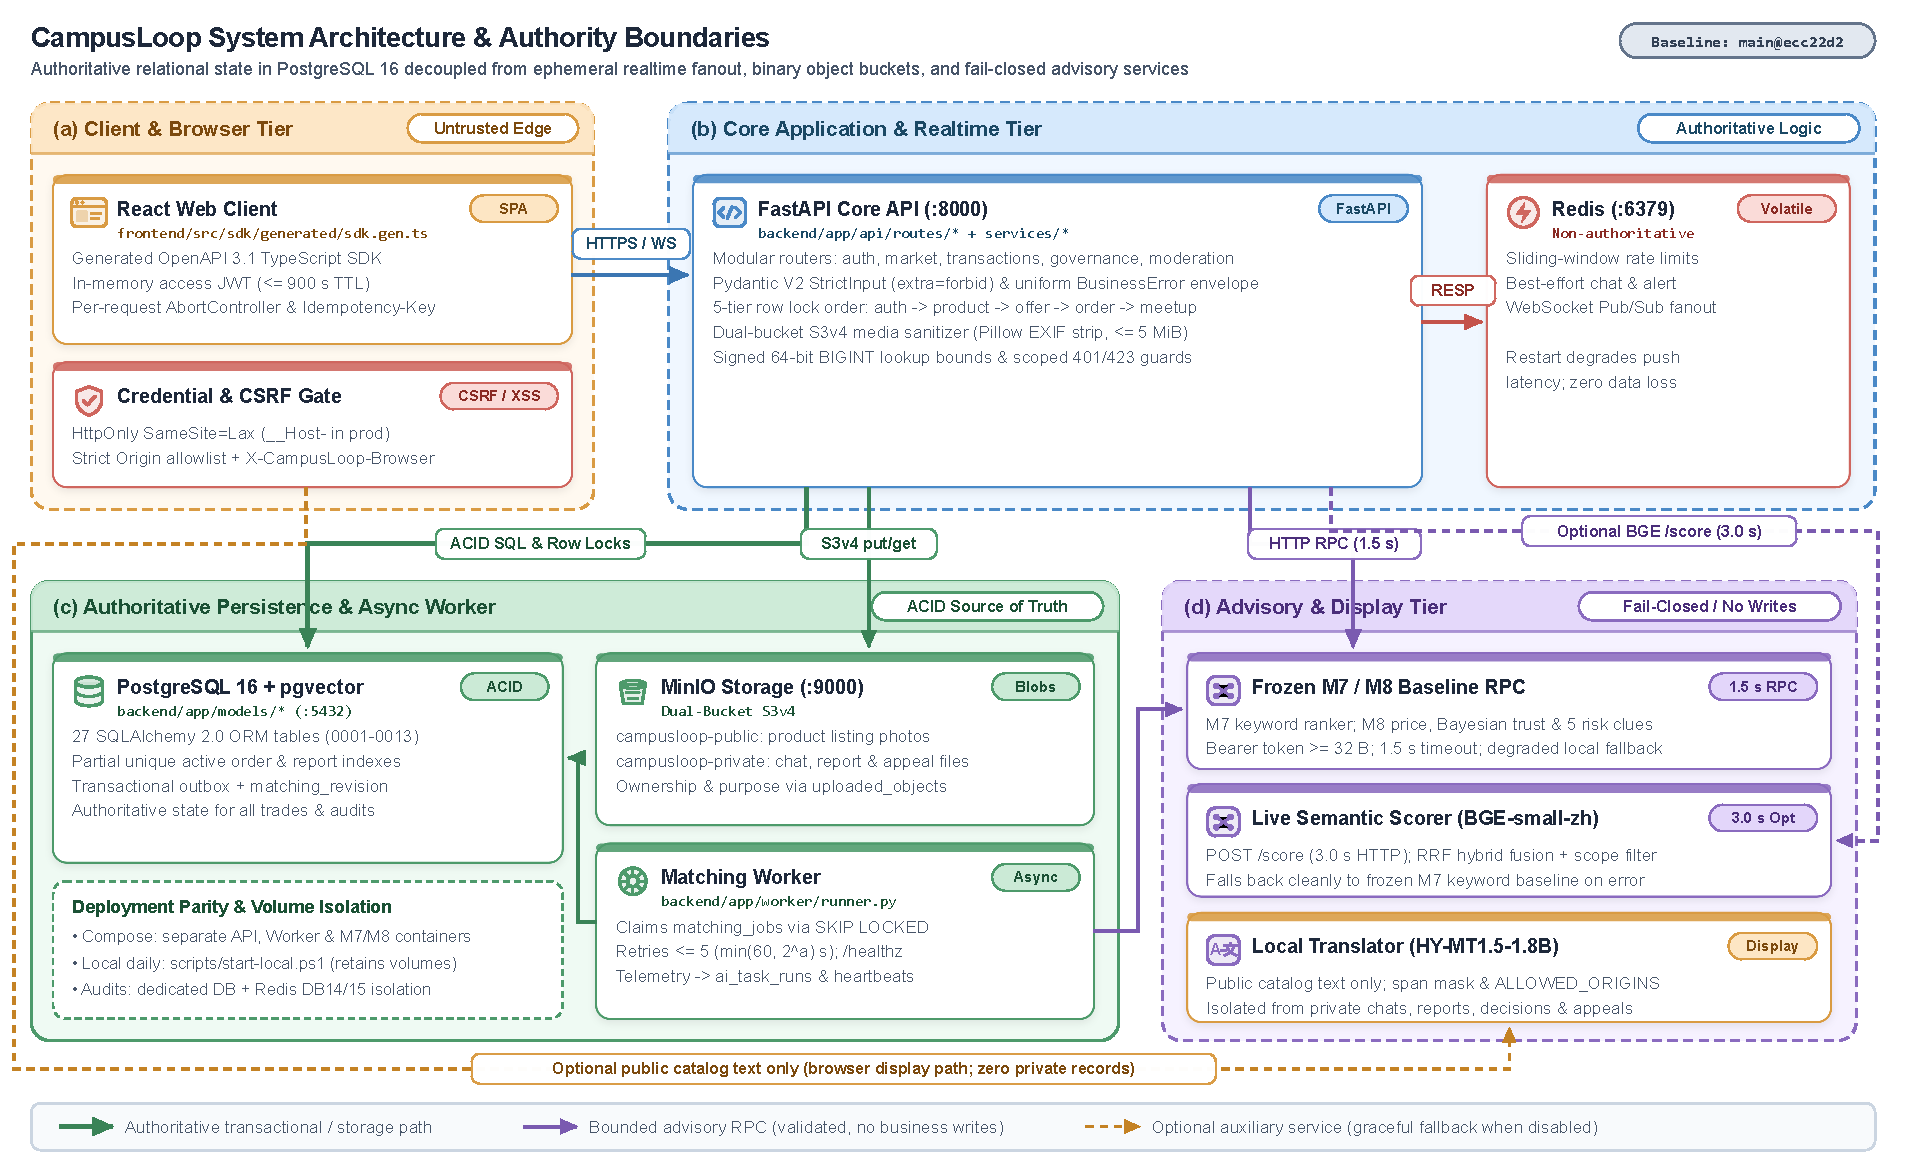
\includegraphics[width=\textwidth]{figures/design/architecture.pdf}
  \caption{CampusLoop runtime architecture and trust boundary.}
  \label{fig:architecture}
\end{figure}

This separation keeps advisory failures out of transaction updates. A timeout or malformed response from an advisory service must not mutate a product, accept an offer, complete an order, or resolve a report. The API performs business updates and commits them through PostgreSQL transactions. The repository's deployment configuration runs the API, worker, and advisory service as separate processes, with PostgreSQL, Redis, and MinIO as supporting services.

\section{Domain and Data Model}

The backend uses object-relational mapping (ORM) to describe database records as Python classes. Several classes share their timestamp columns through a Python mixin, consistent with SQLAlchemy's documented declarative-mixin mechanism~\cite{r2Mixins}. Class inheritance describes how the code reuses these attributes; foreign-key relationships describe how saved records refer to one another. The diagrams show these as separate relationships.

The data model follows the transaction journey. A \emph{User} owns products and wanted posts. A product or wanted post gives a two-party chat session its context, so a conversation remains linked to the item or request being discussed. Offers belong to that session. Accepting an offer creates an order for the referenced product, and the order retains its state history and at most one current meetup arrangement. A review can be submitted only after the transaction is completed.

Governance records serve a different purpose. A report refers to a user, product, order, or chat message and stores the reporter, evidence keys, resolution, handler, and timestamps. Separate AccountDecision and AccountAppeal records let students see account-handling decisions and request review without exposing private report contents.

The entity relationship diagram (ERD) is divided into catalog/chat, transaction, and governance views so that these relationships can be read without crowding one figure. Figure~\ref{fig:data-model} introduces the catalog and chat records. The figures show selected columns; the companion model/migration inventory gives all mapped columns, declared types, and migration constraints. Each record still has its own ownership and state rules.

\begin{figure}[htbp]
  \centering
  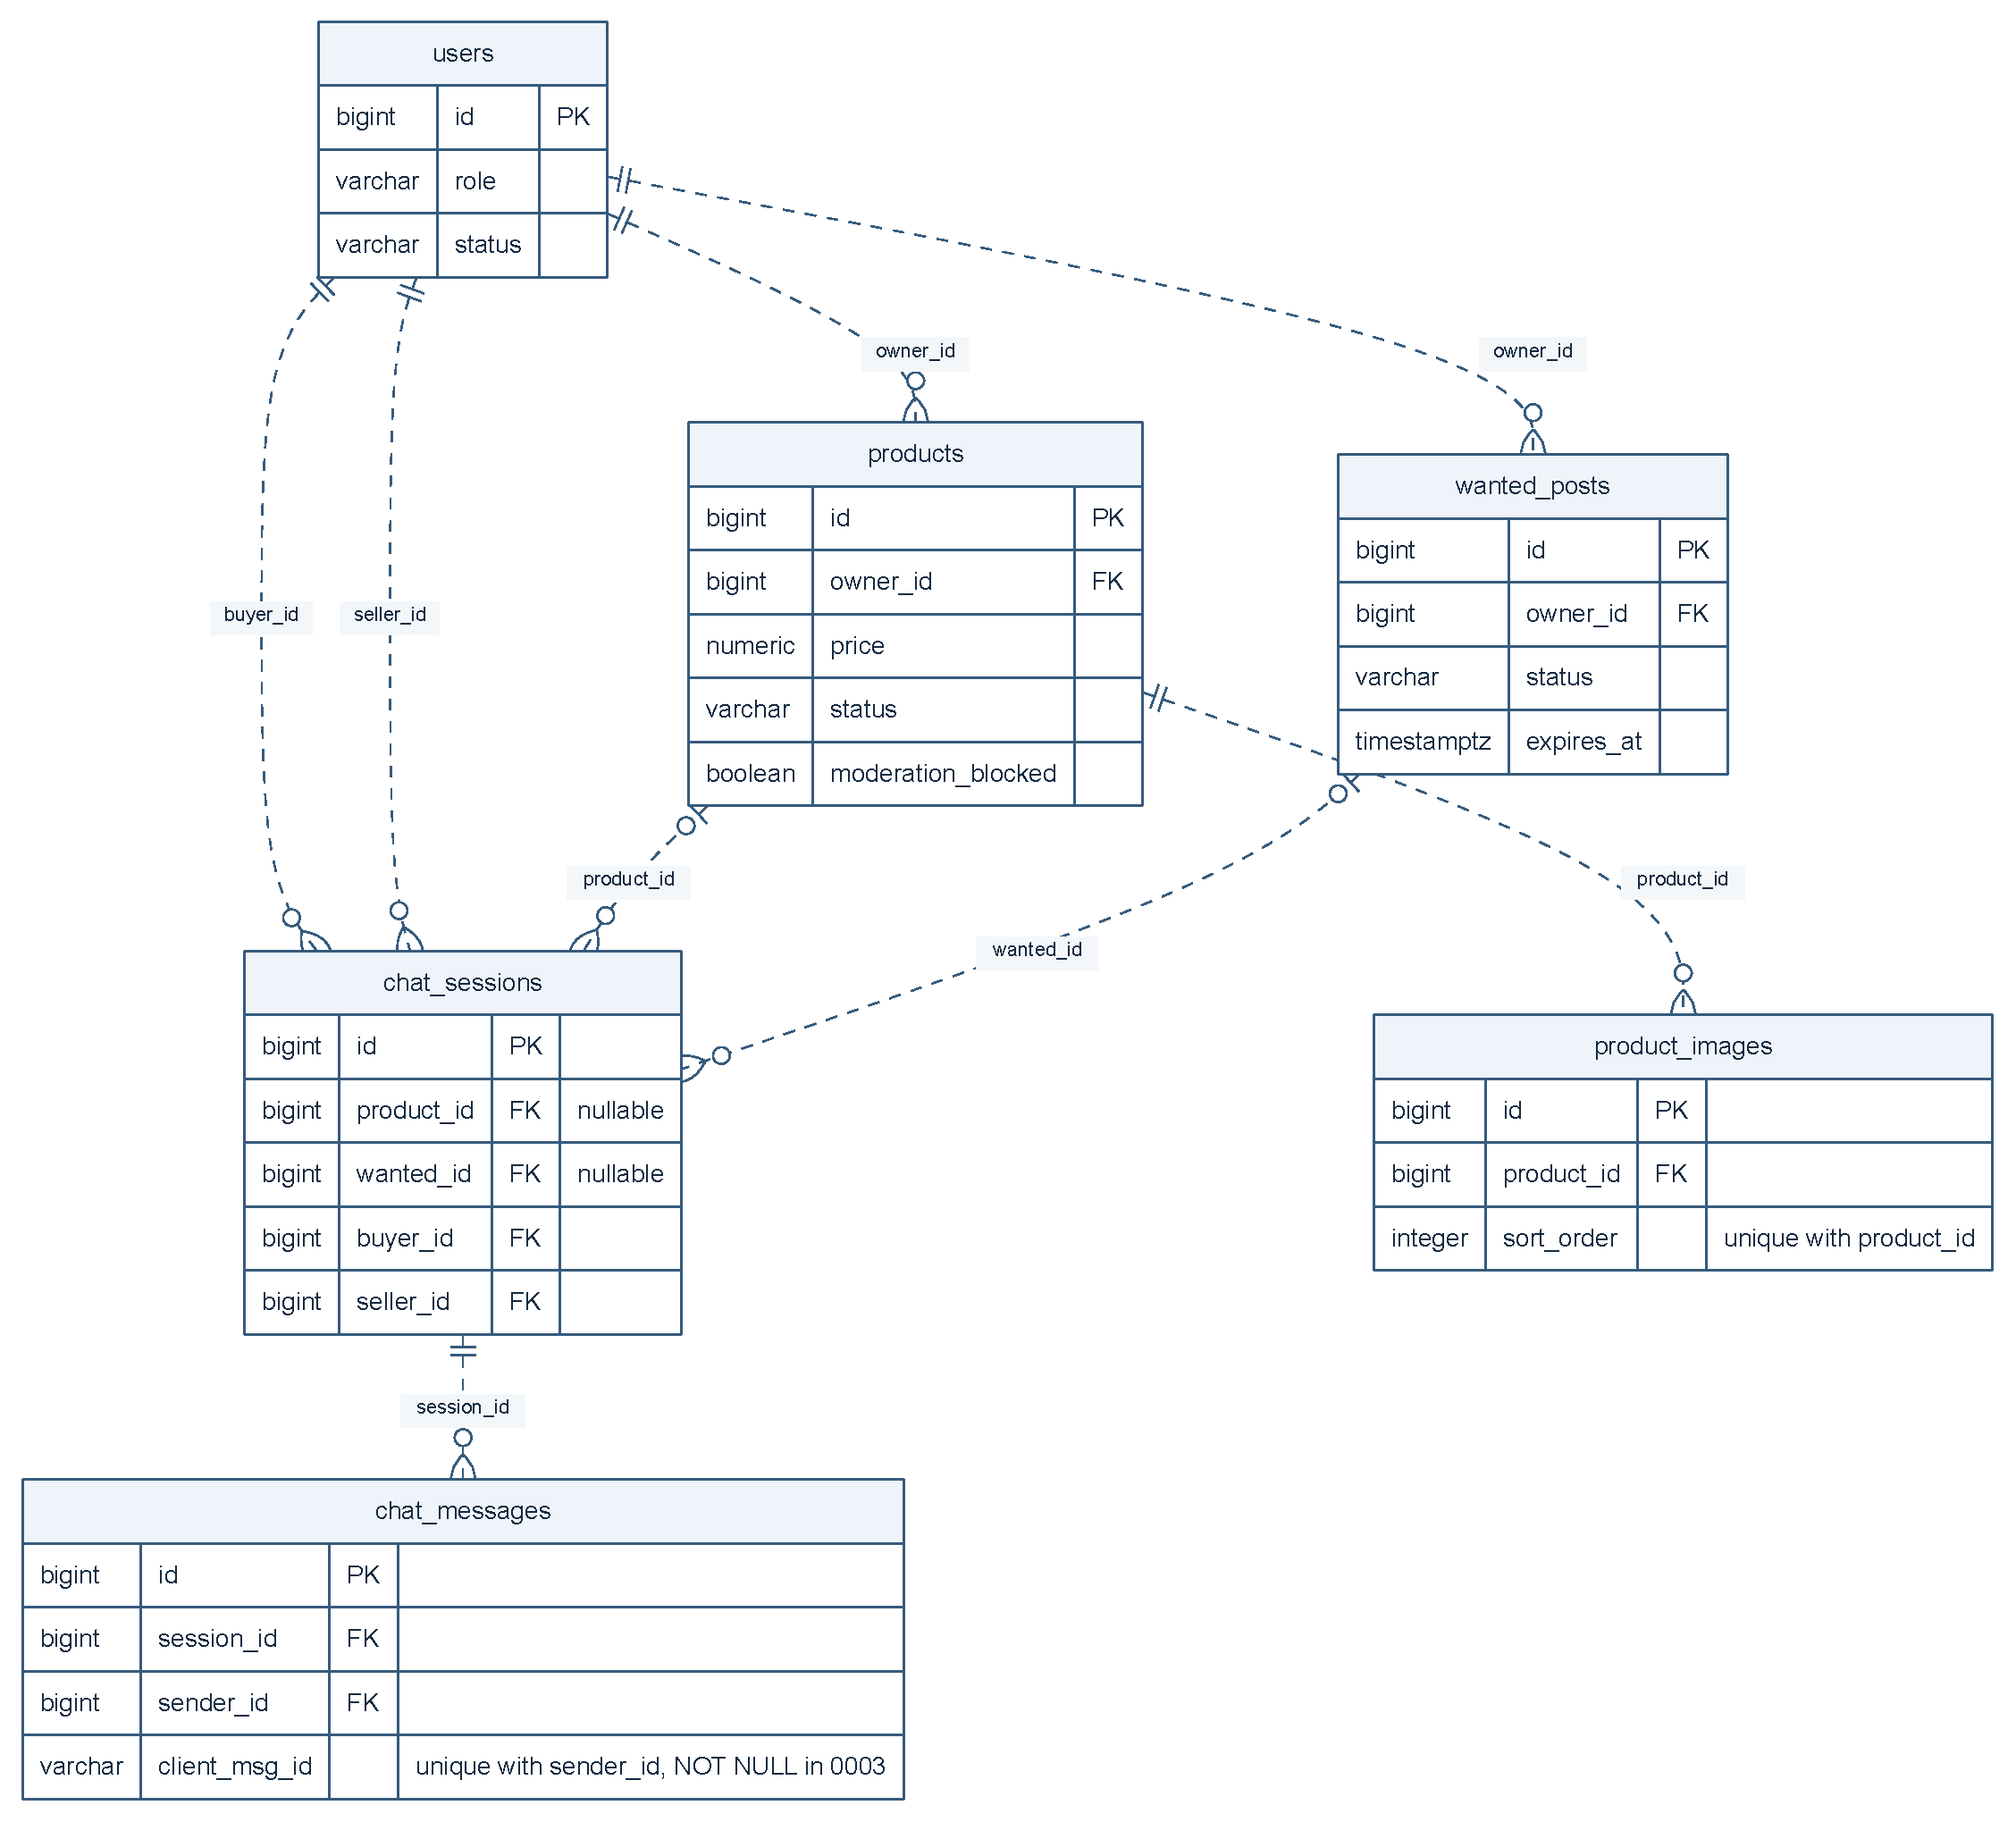
\includegraphics[width=\textwidth]{figures/design/data-model.pdf}
  \caption{Principal persistent entities and relationships.}
  \label{fig:data-model}
\end{figure}

Authentication records are separated from the user profile. A session family groups rotating refresh sessions and allows family-wide revocation after logout or replay detection. Matching jobs and matching results are also separate from live product records. The API therefore checks the live catalog for visibility and entity versions before returning ranked products.

\begin{figure}[p]
  \centering
  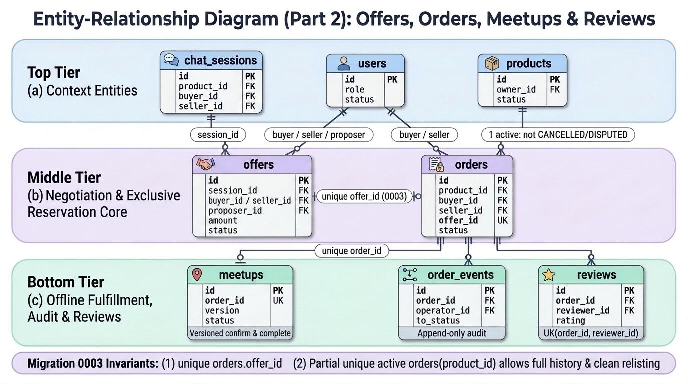
\includegraphics[width=\textwidth,height=0.8\textheight,keepaspectratio]{figures/design/data-model-transactions.pdf}
  \caption{Transaction ERD: historical orders and conditional reservation uniqueness.}
  \label{fig:erd-transactions}
\end{figure}
\begin{figure}[p]
  \centering
  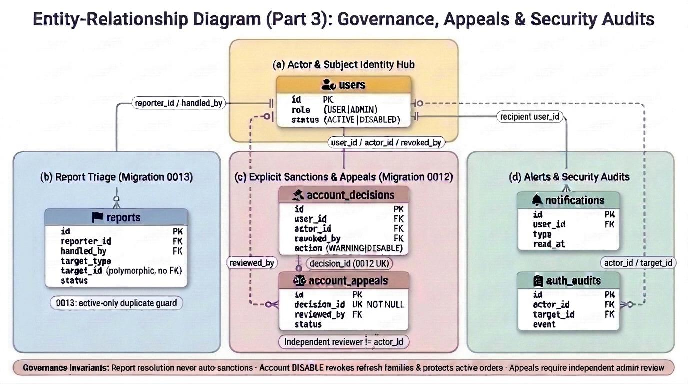
\includegraphics[width=\textwidth,height=0.8\textheight,keepaspectratio]{figures/design/data-model-governance.pdf}
  \caption{Governance ERD: reports, account decisions, appeals, and notifications.}
  \label{fig:erd-governance}
\end{figure}
\begin{figure}[p]
  \centering
  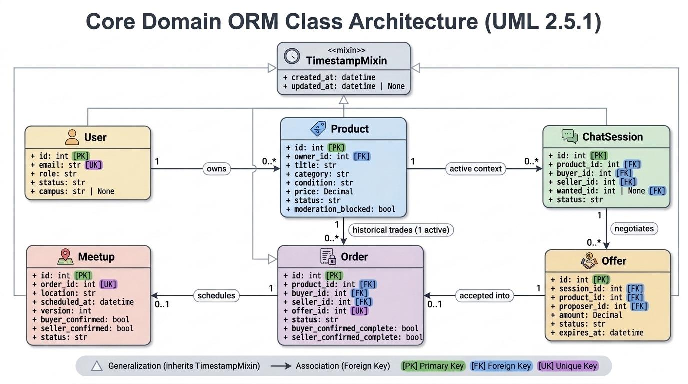
\includegraphics[width=\textwidth,height=0.8\textheight,keepaspectratio]{figures/design/class-diagram.pdf}
  \caption{Selected real ORM classes and their TimestampMixin inheritance.}
  \label{fig:class-diagram}
\end{figure}

Figures~\ref{fig:erd-transactions} and~\ref{fig:erd-governance} separate trading constraints from moderation records. Dashed Crow's Foot relationships are non-identifying foreign-key associations; circles mean optional participation and bars mean one. The class diagram in Figure~\ref{fig:class-diagram} shows selected mapped attributes and inheritance. Database constraints are recorded in the ERD and source inventory. Solid associations denote foreign-key references, not SQLAlchemy relationship objects. The selected classes declare no domain methods, so their diagram entries list attributes only. The source index records the exact definitions and the still-pending course-Lecture notation check.

\section{Authorization Boundaries}

The permission checks follow the relationship between a user and a record. A seller may edit an eligible product they own, while a conversation or order is accessible only to its participants. This means that being signed in does not give a user access to every record in the system.

These rules are enforced in backend routes and services. Student-only updates reject disabled or non-student actors. Product editing requires ownership and excludes reserved, sold, deleted, or moderated listings. Chat reads and writes require the actor to be either the buyer or seller, and wanted-match results are visible only to the wanted-post owner. Order operations require a participant; risk clues and report resolution require an administrator. Private files are read through authenticated API paths, while product media is placed in the public-read bucket.

The authentication path restores browser identity as follows. Login creates a server-side session family and returns an access token while the browser retains an opaque, HttpOnly cookie. On a page reload, the client calls \texttt{restoreBrowserSession}; the server validates the browser origin and cookie, applies the refresh window, records an audit event, and returns a new short-lived access token and current-user view. Refresh-token replay revokes the entire family before the API returns an authentication error.

\begin{figure}[htbp]
  \centering
  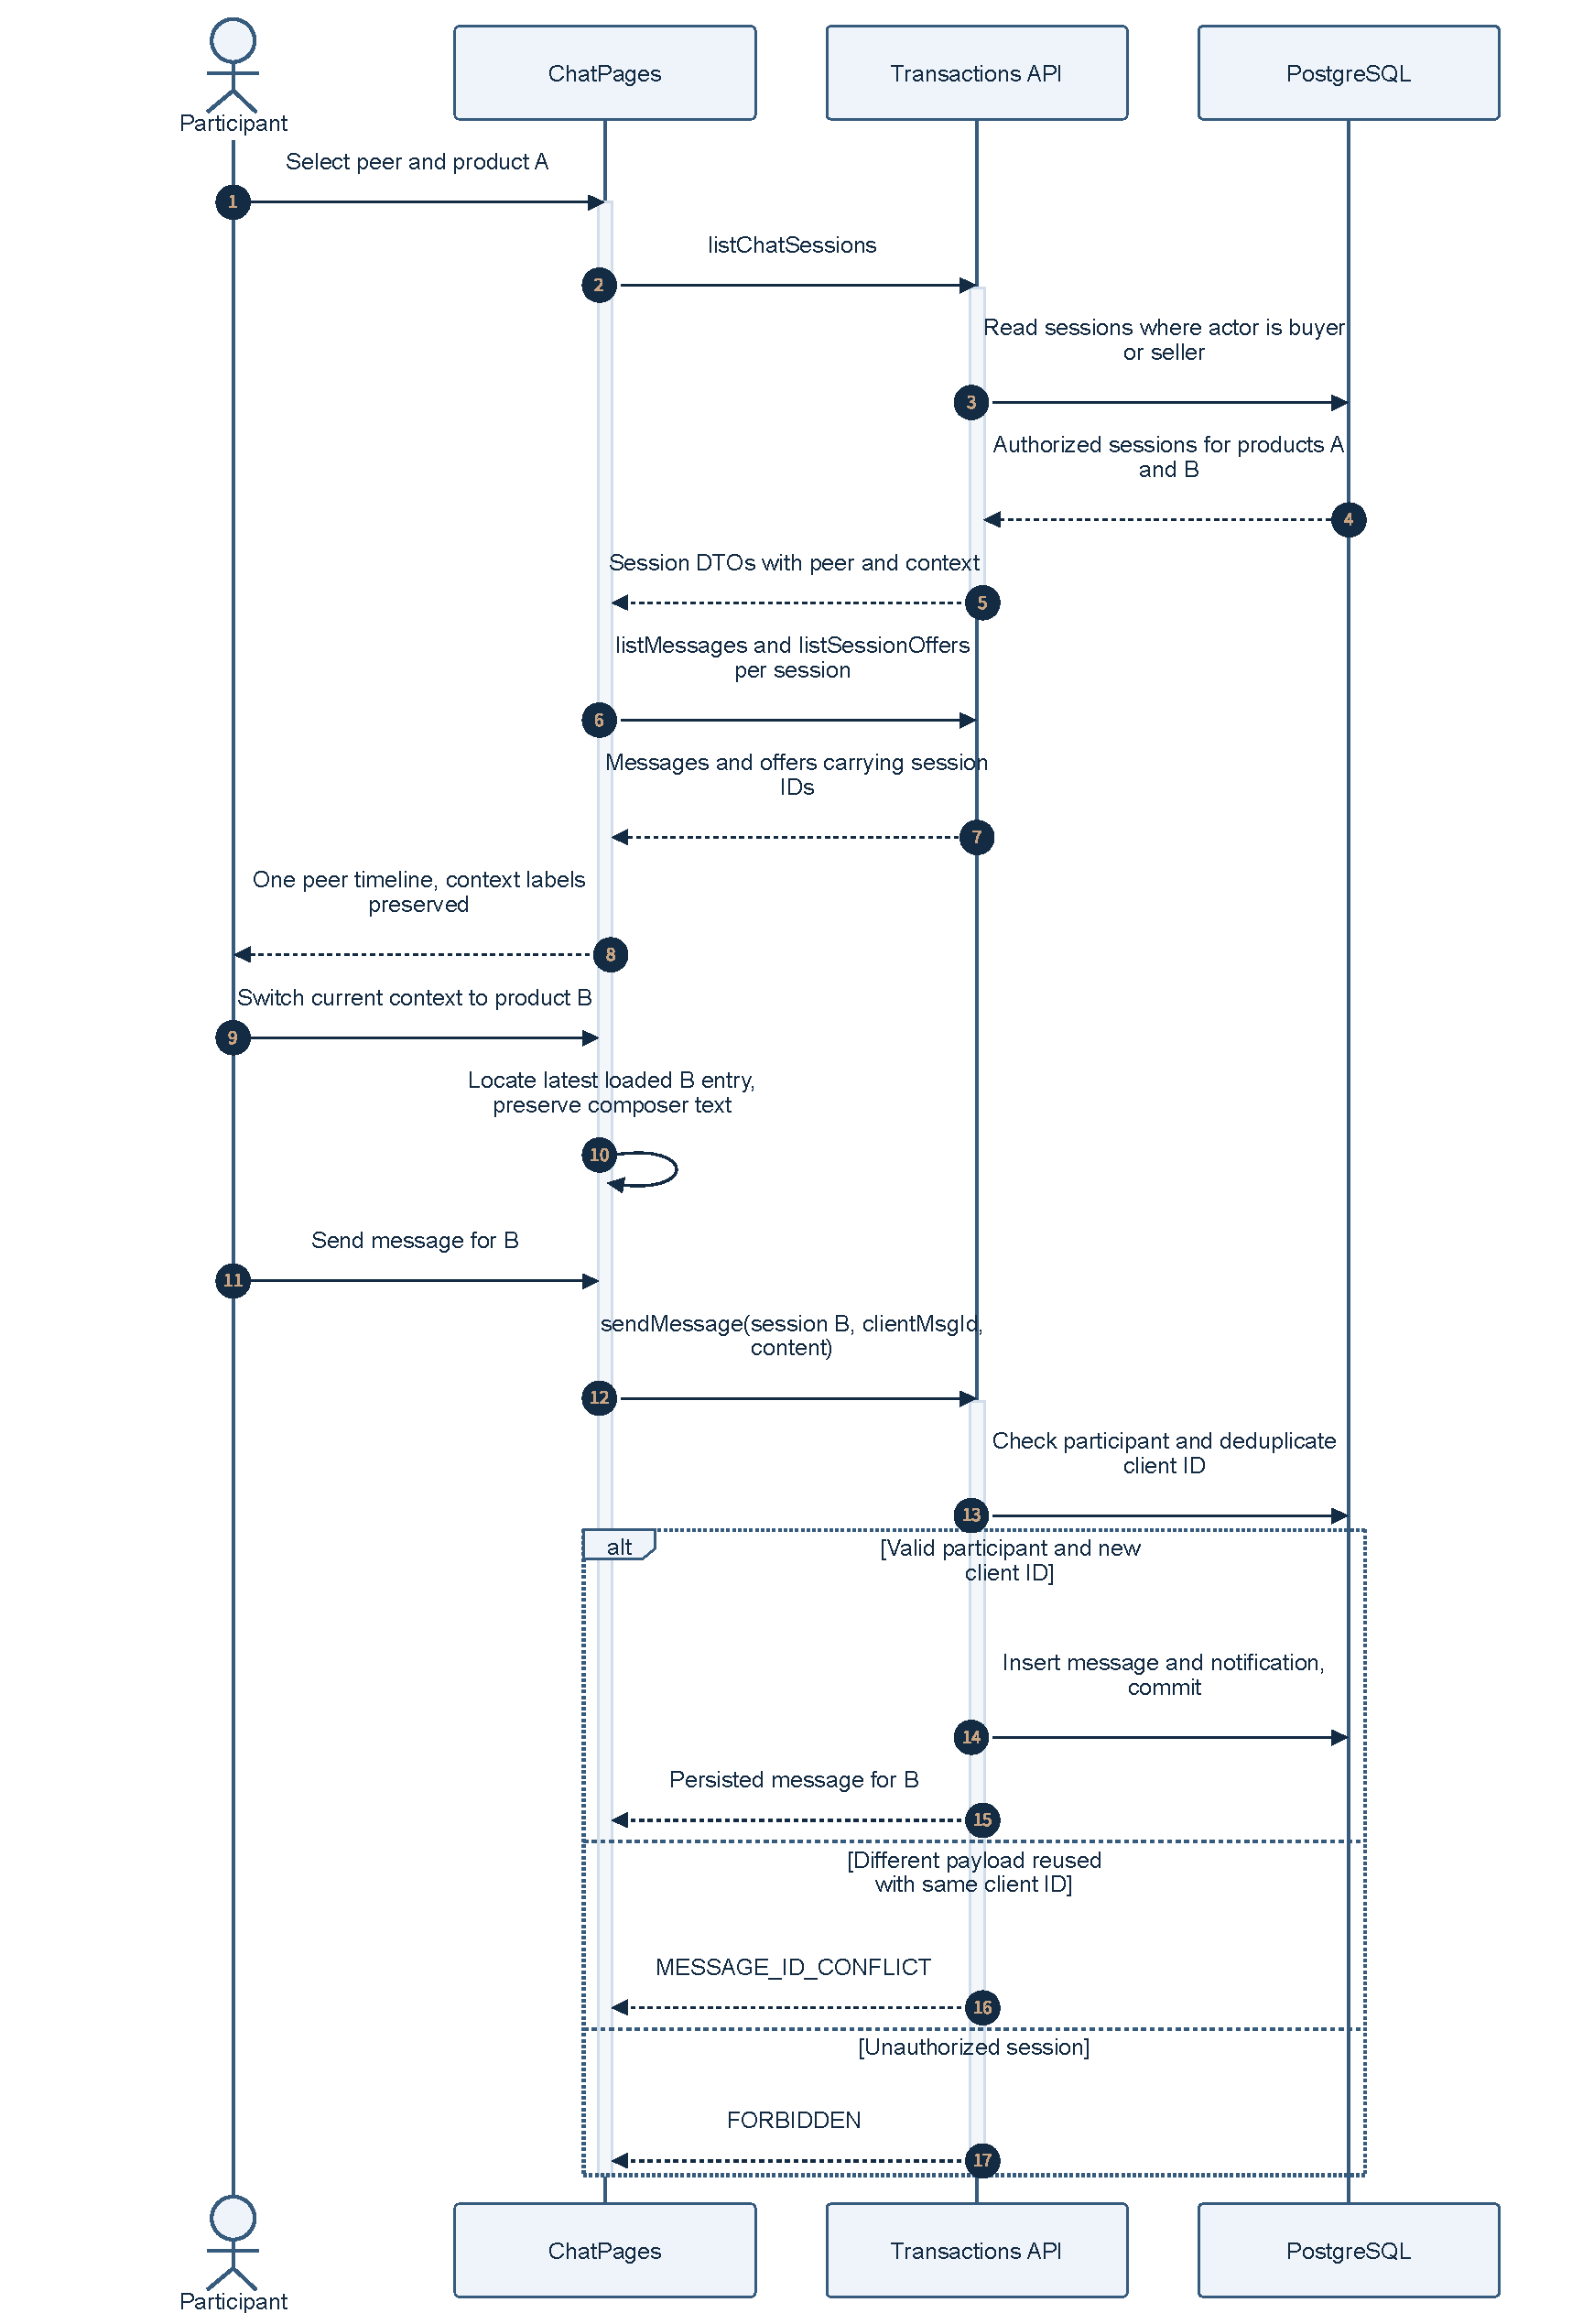
\includegraphics[width=0.94\textwidth]{figures/design/session-sequence.pdf}
  \caption{One peer timeline retaining separate product-session identities.}
  \label{fig:session-sequence}
\end{figure}

\section{Transaction State Machine}

A transaction changes both the order and the availability of the product. The API therefore updates their states together. When a pending offer is accepted under row locks, the product changes from \texttt{ON\_SALE} to \texttt{RESERVED}, and a new order enters \texttt{PENDING\_CONFIRM}. The reservation records that the item is involved in an agreed transaction, although the meeting and completion steps are still outstanding.

The participants then agree on a meetup proposal. Its version increases whenever the proposal changes, and a change resets both meetup confirmations and both completion confirmations. This matters because confirming an earlier time or place should not count as accepting a revised arrangement. The order reaches \texttt{MEETUP\_ARRANGED} only after both participants confirm the same version. It reaches \texttt{COMPLETED} only after both confirm completion against that version, at which point the product becomes \texttt{SOLD}. Figure~\ref{fig:transaction-states} shows this path.

\begin{figure}[htbp]
  \centering
  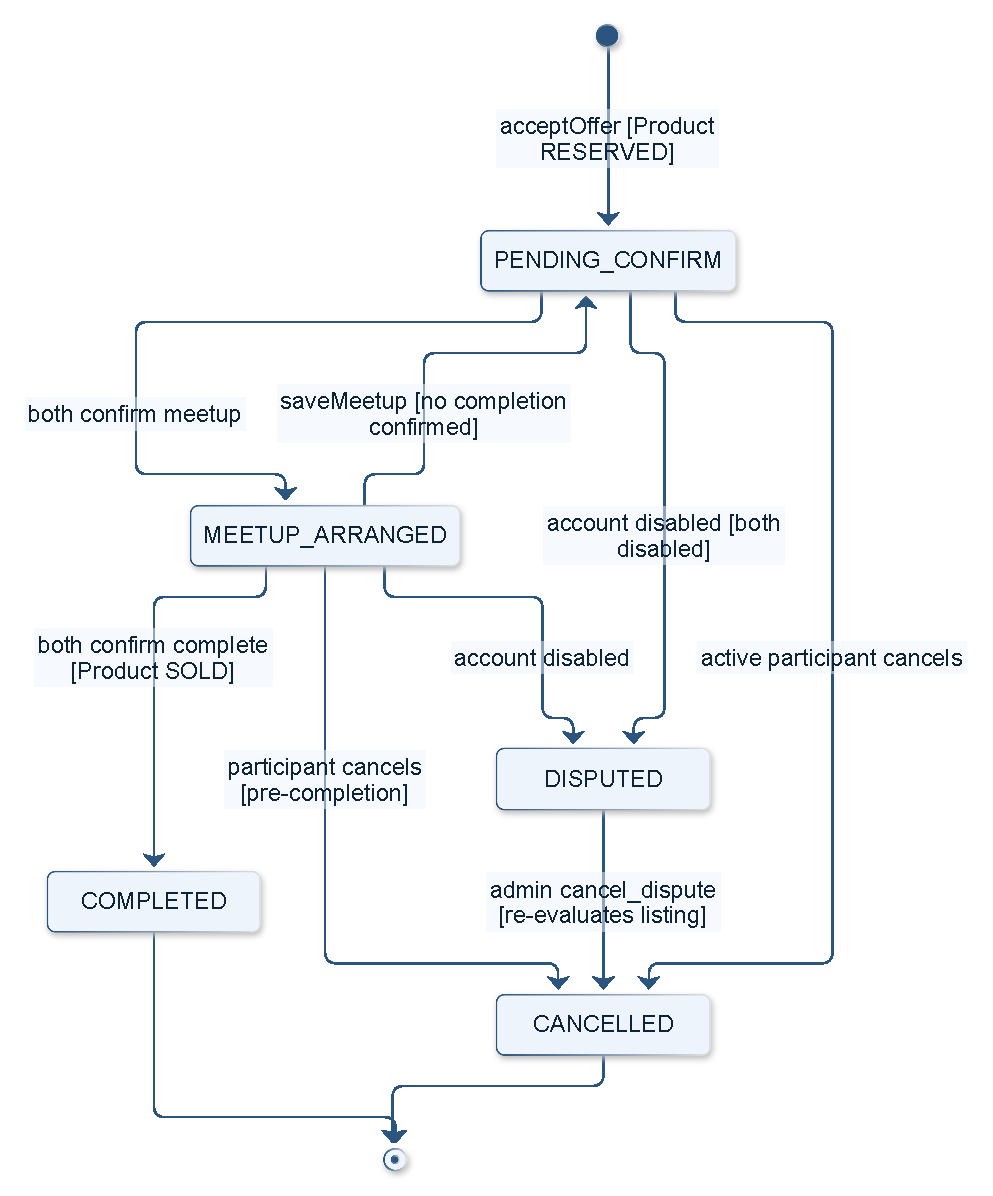
\includegraphics[width=0.94\textwidth]{figures/design/transaction-states.pdf}
  \caption{Coordinated listing, order, meetup, and completion states.}
  \label{fig:transaction-states}
\end{figure}

Cancellation depends on the order's state and confirmation flags. Once either participant has confirmed completion, cancellation is rejected. Before that point, cancellation releases an eligible listing back to \texttt{ON\_SALE}; a deleted or moderation-blocked listing remains \texttt{HIDDEN}. Every order transition appends an \texttt{OrderEvent}, preserving who acted, the before/after state, a description, and a timestamp. Figure~\ref{fig:order-meetup-sequence} shows the complete negotiation-to-completion interaction.

\begin{figure}[htbp]
  \centering
  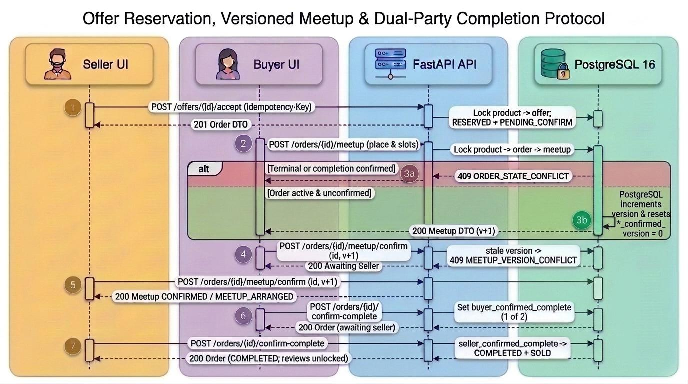
\includegraphics[width=\textwidth]{figures/design/order-meetup-sequence.pdf}
  \caption{Offer acceptance, versioned meetup agreement, and dual completion confirmation.}
  \label{fig:order-meetup-sequence}
\end{figure}

\section{Governance Design}

A report is a request for human review, not an automatic sanction. The reporting route prevents self-reporting, verifies that an order or chat-message reporter is a participant, verifies media ownership, and rejects a duplicate open report with the same reporter, target, and reason. Resolution is restricted to administrators. A normal decision accepts only pending or processing reports; changing a completed decision requires an explicit override containing the status and handling timestamp last observed by the administrator. The server compares those values with the saved record. A stale browser cannot overwrite a newer decision.

Each resolution saves the handler, time, required note, and resulting status. It also notifies the reporter and writes an audit event with before and after snapshots. The event explicitly records \texttt{enforcementExecuted=false}; the present implementation resolves the report record but does not claim that a user or listing sanction was automatically executed.

\section{Explicit Account Handling and Appeals}

Resolving a report records what an administrator decided about that report. Issuing a warning or disabling a student account is a separate action, which requires a reason, facts, and policy basis. Keeping these commands separate makes it possible to record the report outcome without silently treating it as an account sanction.

Disabling an account also affects transactions already in progress. The system revokes transaction sessions and protects the affected orders. Orders with a confirmed meetup or a completion confirmation move to dispute; earlier reservations remain available for controlled cancellation by an active participant. This treatment reflects the difference between an early reservation and a transaction where a participant may already have acted on an agreed meeting.

A student whose trading access is disabled can still use restricted appeal access to read the disclosed decision snapshot and submit an appeal. Another administrator normally reviews it. The development environment has an explicitly configured single-administrator exception, but its use is audited and does not count as independent review. If the account is reinstated, the original decision history remains, and disputed transactions are not automatically resolved.

\section{Traceability Baseline}

All claims in Chapters~\ref{chap:design}--\ref{chap:decisions} were checked against repository commit \texttt{edb9e32871eac2966750993294078acbfdba65f9}. The companion \texttt{architecture-source-index.md} maps every diagram and source chain to concrete routes, services, models, frontend calls, and deployment definitions. Using one fixed baseline keeps the chapter descriptions tied to the same version of the software.

\chapter{System Implementation}
\label{ch:implementation}

This chapter describes how CampusLoop translates the architectural design of Chapter~\ref{ch:design} into concrete frontend, backend, persistence, worker, media, and deployment mechanisms. All module paths, function names, HTTP contracts, concurrency locks, and error codes reflect the verified codebase at \texttt{main@ecc22d2}.

\begin{clbox}{Implementation Pillars and Hardening Summary}
  \small
  \begin{itemize}[leftmargin=1.2em,itemsep=1pt,topsep=2pt]
    \item \textbf{End-to-end contract safety}: OpenAPI~3.1-generated TypeScript SDK paired with Pydantic~V2 \texttt{StrictInput}, uniform \texttt{BusinessError} envelopes, and signed 64-bit \texttt{BIGINT} bounds.
    \item \textbf{Deterministic concurrency}: five-tier row-lock ordering, \texttt{Idempotency-Key} payload hash verification, and transactional SQLAlchemy outbox hooks consumed via \texttt{SKIP LOCKED}.
    \item \textbf{Defense-in-depth media \& ops}: Pillow EXIF stripping and CRC validation into dual MinIO buckets, isolated audit databases, and public-only \texttt{HY-MT1.5-1.8B} catalog translation.
  \end{itemize}
\end{clbox}

\section{Frontend Architecture and Typed OpenAPI SDK Layer}
\label{sec:impl-frontend}

The web frontend (\texttt{frontend/src/}) is built with React and TypeScript \cite{reactDocs}, structured so that UI pages never assemble raw HTTP requests or hand-maintain response DTOs. Instead, the FastAPI backend exports its OpenAPI~3.1 specification \cite{openapi31}, from which \texttt{frontend/src/sdk/generated/sdk.gen.ts} and its accompanying TypeScript definitions are generated. A thin runtime wrapper in \texttt{frontend/src/sdk/index.ts} layers session management, automatic token refresh, idempotency headers, and error normalization over the generated client.

Key client-side reliability and security mechanisms implemented in \texttt{frontend/src/} include:
\begin{itemize}
  \item \textbf{In-memory identity restoration}: on initial page load, \texttt{restoreIdentity()} invokes \texttt{restoreBrowserSession} using the browser's \texttt{HttpOnly} refresh cookie together with the \texttt{X-CampusLoop-Browser} header, hydrating a short-lived access token strictly in JavaScript memory.
  \item \textbf{Scoped error and lock-out handling}: response interceptors in \texttt{sdk/index.ts} trigger local session cleanup on \texttt{401} or \texttt{423} only for authenticated or session-management requests (\texttt{sessionRequest || authenticationRequest}), preventing unauthenticated public fetches or third-party checks from spuriously clearing an active session.
  \item \textbf{Per-request cancellation and safe retry keys}: the \texttt{useRemote} hook attaches a fresh \texttt{AbortController} to every query so rapidly changing filters or route navigations cannot overwrite newer state with stale responses. Mutating forms use \texttt{useAttemptKey()} to bind a stable \texttt{Idempotency-Key} across retries of the same submission and explicitly call \texttt{reset()} once the operation succeeds so subsequent distinct edits obtain fresh keys.
  \item \textbf{Loop-free navigation}: \texttt{BackLink.tsx} sanitizes return paths by stripping URL fragments, rejecting external origins, preventing cycles, and capping navigation chain depth at eight entries.
\end{itemize}

\section{Backend API Layer, Validation, and Error Contracts}
\label{sec:impl-backend}

The backend (\texttt{backend/app/}) exposes modular FastAPI routers under \texttt{backend/app/\allowbreak api/\allowbreak routes/}: \texttt{auth.py}, \texttt{market.py}, \texttt{transactions.py}, \texttt{governance.py}, \texttt{moderation.py}, \texttt{admin\_\allowbreak console.py}, \texttt{intelligence.py}, and \texttt{realtime.py}. Every request body inherits from a shared Pydantic~V2 strict schema (\texttt{StrictInput}, configured with \texttt{extra="forbid"}) \cite{pydanticDocs} so unexpected client properties fail early with HTTP~\texttt{422} rather than being silently ignored.

All domain and validation errors funnel through \texttt{BusinessError} in \texttt{backend/app/\allowbreak core/\allowbreak errors.py}, returning a uniform JSON envelope containing a machine-readable error code (such as \texttt{AUTH\_\allowbreak ACCESS\_\allowbreak EXPIRED}, \texttt{MESSAGE\_\allowbreak ID\_\allowbreak CONFLICT}, \texttt{MEETUP\_\allowbreak VERSION\_\allowbreak CONFLICT}, \texttt{ORDER\_\allowbreak STATE\_\allowbreak CONFLICT}, or \texttt{INDEPENDENT\_\allowbreak REVIEW\_\allowbreak REQUIRED}) and human-readable message. Path-parameter lookups routed through \texttt{load()} enforce PostgreSQL signed 64-bit \texttt{BIGINT} range bounds ($1 \le \text{id} \le 2^{63}-1$) before querying the database, mapping out-of-range integers cleanly to \texttt{404 NOT\_FOUND} instead of raising unhandled database driver exceptions.

\section{End-to-End Source Chains}
\label{sec:impl-chains}

To provide direct code traceability across the full stack, Table~\ref{tab:source-chains} maps six core user and administrative workflows from React UI components through generated SDK operations and FastAPI route/service handlers to authoritative PostgreSQL tables and failure boundaries.

\begin{table}[htbp]
  \centering
  \footnotesize
  \setlength{\tabcolsep}{4pt}
  \renewcommand{\arraystretch}{1.12}
  \caption{Six end-to-end source chains verified at \texttt{main@ecc22d2}.}
  \label{tab:source-chains}
  \begin{tabularx}{\linewidth}{@{}>{\raggedright\arraybackslash}p{2.2cm}>{\raggedright\arraybackslash}p{4.7cm}>{\raggedright\arraybackslash}p{3.0cm}>{\raggedright\arraybackslash}X@{}}
    \toprule[1pt]
    \cltblhdr \textbf{\color{clNavy}Workflow} & \textbf{\color{clNavy}UI $\to$ SDK $\to$ Backend Handler} & \textbf{\color{clNavy}Persisted Tables} & \textbf{\color{clNavy}Primary Boundary / Guard} \\
    \midrule
    1. Browser Session & \texttt{AccountPages.tsx}, \texttt{sdk/index.ts} $\to$ \texttt{login}, \texttt{refreshSession}, \texttt{restoreBrowser\allowbreak Session} $\to$ \texttt{auth.py}, \texttt{services/auth.py} & \texttt{users}, \texttt{auth\_session\_\allowbreak families}, \texttt{refresh\_\allowbreak sessions}, \texttt{auth\_audits} & Rejects untrusted \texttt{Origin} or missing CSRF header; revokes full family on replay; expired token fails \texttt{401} before appeal check. \\
    2. Listing Publish & \texttt{MarketPages.tsx}, \texttt{ImageQueue.tsx} $\to$ \texttt{uploadImage}, \texttt{createProduct} $\to$ \texttt{market.py}, \texttt{services/storage.py} & \texttt{uploaded\_\allowbreak objects}, \texttt{products}, \texttt{product\_\allowbreak images}, \texttt{idempotency\_\allowbreak records} & Validates MIME/pixels/EXIF; enforces \texttt{owned\_keys} ownership \& purpose; conflicts on mutated idempotency replay. \\
    3. Chat \& Offer & \texttt{ChatPages.tsx} $\to$ \texttt{createChatSession}, \texttt{listMessages}, \texttt{sendMessage}, \texttt{createOffer} $\to$ \texttt{transactions.py} & \texttt{chat\_sessions}, \texttt{chat\_\allowbreak messages}, \texttt{offers}, \texttt{notifications} & Blocks self-contact; checks participant; enforces \texttt{MESSAGE\_ID\_\allowbreak CONFLICT}; dynamically marks past-expiry offers \texttt{EXPIRED}. \\
    4. Unique Reserve & \texttt{ChatPages.tsx} $\to$ \texttt{acceptOffer} $\to$ \texttt{transactions.py::\allowbreak accept\_offer} & \texttt{offers}, \texttt{products}, \texttt{orders}, \texttt{order\_events}, \texttt{idempotency\_\allowbreak records} & Blocks self-acceptance; locks \texttt{product -> offer}; Migration~\texttt{0003} unique \texttt{offer\_id} \& partial active \texttt{product\_id} index. \\
    5. Meetup \& Review & \texttt{TransactionPages.tsx} $\to$ \texttt{saveMeetup}, \texttt{confirmMeetup}, \texttt{confirmOrder\allowbreak Complete}, \texttt{createReview} $\to$ \texttt{transactions.py} & \texttt{meetups}, \texttt{orders}, \texttt{order\_events}, \texttt{products}, \texttt{reviews} & Rejects stale meetup version (\texttt{409}) and post-completion edits (\texttt{409}); dual flags for \texttt{COMPLETED}; allows review even if peer disabled. \\
    6. Governance \& Appeals & \texttt{AdminPages.tsx}, \texttt{AccountDecision\allowbreak Controls.tsx}, \texttt{AppealsPage.tsx}, \texttt{ModerationPages.tsx} $\to$ \texttt{resolveReport}, \texttt{overrideReport}, \texttt{adminCreate\allowbreak AccountDecision}, \texttt{submitAccount\allowbreak Appeal}, \texttt{adminReview\allowbreak AccountAppeal} $\to$ \texttt{governance.py}, \texttt{moderation.py} & \texttt{reports}, \texttt{account\_\allowbreak decisions}, \texttt{account\_\allowbreak appeals}, \texttt{auth\_audits}, \texttt{notifications} & Blocks self-reporting own message; separates triage from sanctions; revokes sessions \& protects orders on disable; enforces independent reviewer. \\
    \bottomrule
  \end{tabularx}
\end{table}

Several subtle operational refinements verified in \texttt{main@ecc22d2} close edge cases discovered during end-to-end auditing:
\begin{itemize}
  \item \textbf{Closing offers under state transitions}: \texttt{cancel\_offer} and \texttt{reject\_offer} pass \texttt{closing=True} when loading the target offer, enabling participants to cleanly close lingering \texttt{PENDING} offers even after the underlying product has been \texttt{RESERVED} by another trade or the counterparty's account has been disabled.
  \item \textbf{Dynamic expiry projection}: \texttt{offer\_fields()} dynamically reports any \texttt{PENDING} offer whose \texttt{expires\_at} timestamp has passed as \texttt{EXPIRED} during read serialization, preventing stale pending badges in chat even before a write touches the row.
  \item \textbf{Post-completion reviews with disabled peers}: \texttt{create\_review} invokes participant loading with \texttt{allow\_disabled\_peer=True} so an active student who already completed a legitimate transaction is not deprived of the ability to leave feedback if the counterparty is subsequently disabled.
  \item \textbf{Wanted-post expiry filtering}: \texttt{list\_wanted(status="EXPIRED")} includes both explicitly marked \texttt{EXPIRED} rows and \texttt{OPEN} rows whose \texttt{expires\_at} deadline has elapsed, ensuring filter views remain consistent with real clock time.
\end{itemize}

\section{Concurrency Control, Lock Ordering, and Idempotency}
\label{sec:impl-concurrency}

High-contention write paths in CampusLoop---such as two competing offers being accepted against the same listing, a buyer modifying a meetup while the seller confirms it, or an administrator disabling an account with in-flight orders---cannot rely on optimistic UI checks alone. The backend enforces three layered PostgreSQL concurrency guarantees \cite{postgresExplicitLocking}:
\begin{enumerate}
  \item \textbf{Deterministic five-tier row-lock hierarchy}: whenever a transaction locks multiple domain rows via \texttt{SELECT ... FOR UPDATE} (or \texttt{FOR NO KEY UPDATE} / \texttt{FOR SHARE NOWAIT} for read-integrity checks), it acquires locks strictly in the global order
  \[
    \texttt{auth / user} \;\longrightarrow\; \texttt{product} \;\longrightarrow\; \texttt{offer} \;\longrightarrow\; \texttt{order} \;\longrightarrow\; \texttt{meetup}.
  \]
  In particular, \texttt{services/order\_governance.py::protect\_disabled\_orders} sorts affected orders by \texttt{(product\_id, order\_id)} and locks \texttt{Product} before \texttt{Order} and \texttt{Meetup}, eliminating circular deadlock cycles with concurrent student trade mutations.
  \item \textbf{Database uniqueness backstops}: Migration~\texttt{0003} backs application locks with unique indexes on \texttt{orders.offer\_id}, active \texttt{orders.product\_id}, \texttt{meetups.order\_id}, \texttt{reviews(\allowbreak order\_id, reviewer\_id)}, and \texttt{chat\_\allowbreak messages(\allowbreak sender\_id, \allowbreak client\_\allowbreak msg\_id)}. Even if two requests execute across separate API workers, PostgreSQL enforces single-winner atomicity.
  \item \textbf{Request idempotency records}: critical mutating routes accept an \texttt{Idempotency-Key} header persisted in \texttt{idempotency\_records} alongside a canonical SHA-256 hash of the request payload and the serialized HTTP response. Replaying the exact request returns the cached result without duplicating rows; reusing the same key with a different payload fails with \texttt{409 IDEMPOTENCY\_CONFLICT}.
\end{enumerate}

\section{PostgreSQL Outbox Matching Worker and Observability}
\label{sec:impl-worker}

When a student publishes or edits a product, updates a wanted post, or changes account status, CampusLoop asynchronously recomputes matching recommendations for open wanted posts without slowing down the synchronous HTTP request. Rather than introducing a separate message broker that could drift out of sync with SQL transactions, \texttt{backend/app/services/matching\_jobs.py} implements a transactional PostgreSQL outbox pattern using SQLAlchemy session hooks \cite{sqlalchemy20}:
\begin{itemize}
  \item \textbf{Transactional event capture}: a \texttt{before\_flush} listener inspects dirty and new \texttt{Product}, \texttt{WantedPost}, and \texttt{User} instances across an explicit allowlist of business fields. In \texttt{after\_flush\_postexec}, the session increments the singleton \texttt{matching\_revision} counter, computes a deterministic SHA-256 \texttt{business\_event\_key} over normalized field values and timestamps, and executes an idempotent \texttt{INSERT ... ON CONFLICT DO NOTHING} into \texttt{matching\_jobs} for every active, non-expired \texttt{WantedPost}. If the enclosing transaction rolls back, \texttt{after\_rollback} clears staged changes so phantom jobs are never emitted.
  \item \textbf{Lock-held job claiming (\texttt{SKIP LOCKED})}: worker processes in \texttt{backend/app/\allowbreak worker/\allowbreak runner.py} claim pending rows via \texttt{SELECT ... FOR UPDATE SKIP LOCKED} \cite{postgresExplicitLocking} and hold the row lock until commit. A crashed worker automatically rolls back its transaction and releases the row lock without requiring lease-expiration sweeps. Failed jobs retry with bounded exponential backoff $\Delta t = \min(60, 2^{a})$ seconds up to \texttt{MAX\_ATTEMPTS = 5} before transitioning to \texttt{FAILED}.
  \item \textbf{Runtime observability}: the standalone worker attaches a \texttt{RunObserver} (\texttt{bp4-worker-\allowbreak runtime-v1}) backed by a bounded 2,000-event in-memory queue that records per-job execution telemetry in \texttt{ai\_task\_runs}, emits throttled heartbeats every 10 seconds to \texttt{worker\_heartbeats}, handles \texttt{SIGTERM}/\texttt{SIGINT} gracefully by draining in-flight commits, and serves live loop status on its internal \texttt{/healthz} HTTP endpoint.
\end{itemize}

\section{Media Security Pipeline and Dual-Bucket Isolation}
\label{sec:impl-media}

User-uploaded images are a common vector for polyglot payloads, decompression bombs, EXIF location leaks, and unauthorized object access. The upload pipeline in \texttt{backend/app/\allowbreak services/\allowbreak storage.py} enforces strict server-side sanitization and ownership isolation before persisting any binary object to MinIO \cite{minioDocs}:
\begin{enumerate}
  \item \textbf{Payload and pixel bounds}: raw uploads exceeding 5~MiB are rejected with \texttt{413 IMAGE\_TOO\_LARGE}. Pillow decodes the buffer in memory, allowing only \texttt{JPEG} and \texttt{PNG} formats whose total pixel count does not exceed $25\times 10^{6}$ pixels, and runs \texttt{image.verify()}.
  \item \textbf{Malicious/corrupted archive rejection}: malformed headers, truncated streams, decompression bombs, and corrupted PNG CRC chunks (\texttt{Unidentified\allowbreak ImageError}, \texttt{OSError}, \texttt{Decompression\allowbreak BombError}, \texttt{SyntaxError}, \texttt{ValueError}, \texttt{EOFError}, and \texttt{zlib.error}) are caught deterministically and mapped to \texttt{415 UNSUPPORTED\_IMAGE}.
  \item \textbf{EXIF stripping and JPEG re-encoding}: valid images are transposed according to EXIF orientation (\texttt{ImageOps.exif\_transpose}), converted to \texttt{RGB}, resized to $512\times 512$ via Lanczos resampling if \texttt{purpose == "avatar"}, and re-encoded into clean \texttt{JPEG} bytes (quality~90), stripping all original EXIF metadata and embedded chunks.
  \item \textbf{Dual-bucket separation and ownership verification}: product photos (\texttt{purpose == "product"}) are stored in \texttt{campusloop-public} under a UUID key; chat attachments, report evidence, decision evidence, and appeal evidence are stored in \texttt{campusloop-private} and assigned non-resolvable internal reference URIs (\texttt{https://private.campusloop.invalid/...}) so browsers can retrieve them only through authenticated FastAPI streaming routes. Every upload writes an \texttt{UploadedObject} row recording \texttt{(owner\_id, object\_key, purpose)}; attaching an image to a listing, message, report, decision, or appeal verifies ownership and purpose via \texttt{owned\_keys()}, rejecting cross-user or cross-purpose object substitution with \texttt{403 FORBIDDEN}. On database commit failure, the uploaded object is deleted in a compensating cleanup path. For appeal evidence specifically, \texttt{uploadAppealImage} verifies that the student currently holds an unrevoked, unappealed \texttt{AccountDecision}.
\end{enumerate}

\section{Runtime Profiles and Local Display Translation}
\label{sec:impl-ops}

To keep daily usage, automated testing, and acceptance audits strictly isolated, CampusLoop maintains separate database and Redis allocations. The local daily startup script (\texttt{scripts/start-local.ps1}) preserves persistent PostgreSQL and MinIO volumes across restarts, whereas write-heavy verification suites target dedicated isolated databases and Redis DB14/DB15 rather than the daily account store.

For bilingual classroom and cross-campus browsing, CampusLoop optionally pairs the web client with a standalone local translation microservice (\texttt{services/\allowbreak catalog\_translation\_\allowbreak server.py}) serving \texttt{HY-MT1.5-1.8B}. To preserve security and reliability boundaries, the translation server enforces four strict controls:
\begin{itemize}
  \item \textbf{CORS and MIME enforcement}: requests must originate from \texttt{ALLOWED\_ORIGINS} and carry \texttt{Content-Type: application/json} with a 10-second socket timeout.
  \item \textbf{Span preservation}: technical model codes, prices, and protected tokens are masked before generation and restored deterministically afterward so model names and currency figures are never hallucinated.
  \item \textbf{Per-item failure isolation}: batch catalog translations execute with \texttt{isolate\_\allowbreak failures=\allowbreak True} so a single problematic string falls back to its original text without aborting the entire listing page.
  \item \textbf{Strict public-text boundary}: only public product titles, descriptions, and search queries are routed to the translator; original database fields remain unchanged, and private chats, moderation facts, reports, and appeals are never transmitted to the translation service.
\end{itemize}

\chapter{Advisory Intelligence Methods and Limitations}
\label{chap:ai-methods}

\section{Safety Boundary}

The intelligence features help users find suitable items and interpret the information available to them. Their value depends both on how the software handles a request and on whether the underlying data supports the advice. This chapter explains those questions separately: it describes the implemented inputs and outputs, then sets out what remains unverified.

CampusLoop treats every intelligence result as advisory. Search ranks visible products; wanted matching proposes candidates; price advice provides a non-binding interval or an unavailable result; trust summarizes completed-review evidence; and risk clues summarize limited observable activity for an administrator. None of these paths may accept an offer, change an order, hide a listing, disable an account, or resolve a report. Figure~\ref{fig:ai-fallback} shows where the system validates inputs, calls services, falls back, and requires human review.

\begin{figure}[htbp]
  \centering
  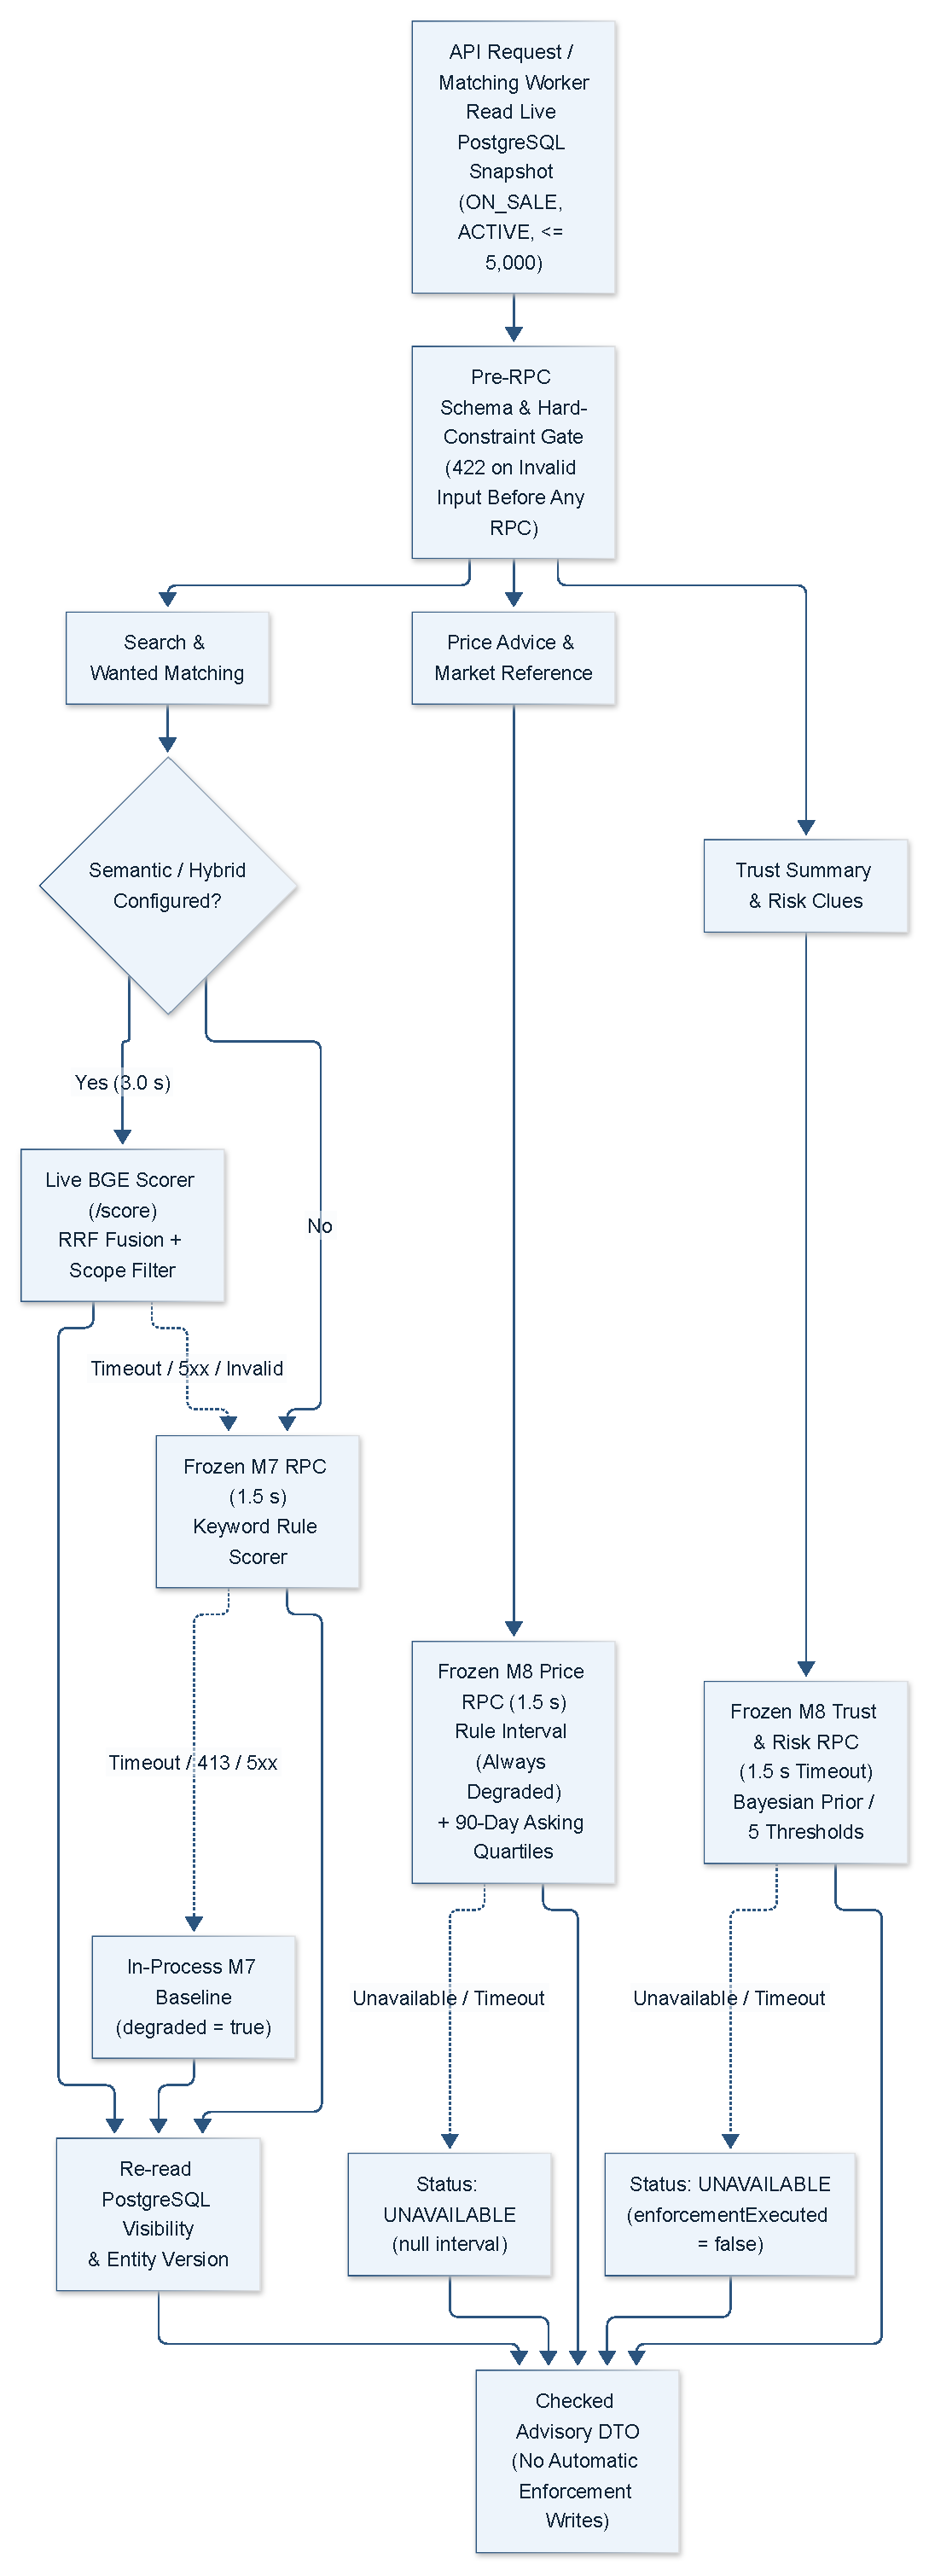
\includegraphics[width=0.92\textwidth]{figures/design/ai-fallback.pdf}
  \caption{Advisory validation, bounded RPC, explicit degradation, and human review.}
  \label{fig:ai-fallback}
\end{figure}

\section{Search and Wanted Matching}

\subsection{Inputs and Output Contract}

Search and wanted matching start from the same eligible catalog. The API takes a snapshot of at most 5,000 products that have not been deleted, are \texttt{ON\_SALE}, and belong to active users. Each candidate contains its stable product and owner identifier, title, description, normalized category and condition, price in fen, campus location, visibility, status, entity version, and publication timestamps.

The request then adds the information needed for the particular task. Search uses the query text, optional category, condition and price filters, mode, and sort order. Wanted matching also uses the wanted-post owner, status, expiry, budget bounds, minimum condition, and required location. These constraints matter because a textually similar product may still be unsuitable for the student's budget or location.

The frozen ranking contract returns product identifiers and versions, a bounded relevance score, deterministic reasons and explanation details, and metadata containing schema, algorithm, dictionary, mode, degradation, and fallback reason. Before exposing results, the API re-reads each ranked product and its owner from PostgreSQL and rejects entries that are no longer public or whose version has changed. A SHA-256 result version covers the stable input snapshot, request, algorithm, options, and requested search mode.

\subsection{Method and Degradation}

Keyword search and wanted matching use the checked-in M7 rule baseline. Optional semantic or hybrid search calls a live semantic service; an unavailable or malformed semantic response is refined by the local catalog-search implementation and marked \texttt{degraded=true} with \texttt{SEMANTIC\_UNAVAILABLE}. The RPC adapter independently computes the frozen rule baseline before accepting a remote result. The adapter checks the response schema and algorithm metadata. It also checks product eligibility, duplicate identifiers, entity versions, score bounds, and exact agreement with the frozen rule explanations. All checks must pass before the response is accepted. Transport failure, timeout, service disablement, or invalid output therefore cannot introduce an unknown candidate.

These checks show whether a response follows the contract. They do not show that its ranking is better. The available evaluation material does not yet include an independently reviewed, representative query set showing an improvement over the original search. Reported ranking quality must therefore be limited to reproducible test outcomes; no production-quality or accuracy claim is made here.

\section{Price Advice}

Price advice receives category, condition, optional original price, title, and description. The current adapter normalizes category and condition, converts original price to fen, and supplies explicit unknown values for purchase age, accessory state, and defect tags. Title and description are not features of the frozen price rule. Title is separately used as a literal keyword for the market-reference query. The frozen M8 service returns a CNY interval, status, explanatory factors, sample size, algorithm version, degradation reason, and disclaimer.

The API accepts the price response only when it follows the frozen \texttt{m8-price-rule-v1} contract. Every current response must be marked as degraded. A result may contain a bounded interval with \texttt{LOW\_CONFIDENCE}, or it may contain no interval with \texttt{INSUFFICIENT\_DATA}/\texttt{UNAVAILABLE}. These statuses tell the interface how much information it can reasonably show.

The same caution applies when the service fails. If it is disabled, times out, becomes unavailable, or returns malformed output, the API returns an unavailable fallback with no interval. The interface must keep manual pricing available and show the disclaimer that the advice does not guarantee a transaction price. The seller therefore remains responsible for choosing the asking price.

The project currently lacks a sufficiently large, authorized set of real completed transactions for training or final evaluation. Synthetic samples test contract behavior but cannot establish market calibration. The system therefore continues to use the rule fallback. The report does not claim that a learned price model has been trained, accepted, or approved for deployment.

\subsection{Live Listing Reference Is Not a Transaction Label}

A separate market reference appears in the same API response. It uses up to 100 recent visible listings from other active sellers. A matching listing must have the same category and condition, a positive price, a title containing a keyword of at least two characters, and a publication date within 90 days. With at least three matches, the reference returns discrete lower and upper quartile listing prices. Otherwise, it leaves the bounds absent. The count is accompanied by up to five source listings, which gives the user some context for the reference.

The distinction between a listing and a completed transaction is essential here. A listing records what a seller asks, not what a buyer eventually pays. These prices therefore do not supply transaction training labels or remove the learned-model NO-GO gate. The seeded 15 demonstration orders also remain synthetic histories; they are useful for demonstrating pages, but cannot be treated as independent real market evidence.

\section{Trust Summary}

The public trust endpoint reads only ratings attached to completed orders. It does not convert an unrated transaction into a five-star event, and it rejects an input history above the explicit capacity limit. The resulting service payload contains review events with completed, non-disputed, valid status and their observed rating. Public serialization is performed through a restricted trust view.

The summary uses only this limited review history. A small number of reviews, selection bias in who submits reviews, coordinated ratings, and context differences between categories can all distort the summary. The value is an aid to judgment, not proof that a user is safe. It must not replace transaction safeguards or governance review.

\section{Administrative Risk Clues}

Risk clues are available only to an administrator who supplies a review reason. The current observable inputs are listing count in the previous hour, distinct chat counterparties in the previous 24 hours, and reports targeting the user or the user's products in the previous seven days. Failed-payment count and same-device account count are explicitly \texttt{null}: the MVP has no payment gateway and does not collect device fingerprints. The response records its source-window timestamp.

Every read is audited with the actor, target, reason, purpose, result status, and \texttt{enforcementExecuted=false}. This records why an administrator inspected the clues and makes clear that viewing them does not itself execute a sanction.

The clues need interpretation. Reports may be false, a new user may have little history, and relevant activity may fall outside the measured windows. Missing signals can also affect the result. These limits can produce false positives or false negatives, so absent inputs remain explicit instead of being replaced with zeroes. The administrator must review the available evidence and take responsibility for any subsequent decision.

\section{Distinct Timeouts and Contracts}

The frozen M7/M8 RPC boundary has a 1.5-second timeout. The optional live semantic scorer uses a separate three-second HTTP timeout and checks its own version, exact candidate identities, finite cosine scores, and hard constraints. It is not admitted through the frozen M7 response validator. The AI flow diagram summarizes these two paths as an engineering flowchart; it does not assert one shared algorithm or one shared timeout. Public catalog translation is another display-only model service and is not evidence of ranking or price accuracy.

\section{Evaluation and Go-Live Gates}

The next evaluation step depends on the task. Search and wanted matching need a frozen, representative query set with independently reviewed relevance labels. The evaluation must retain the baseline and report reproducible metrics so that any claimed improvement can be checked.

Price advice first needs permission to use order data and a documented definition of a valid completed transaction, including how refunds and disputes are handled. The data gate requires at least 200 qualified records and at least 30 records in each key category or price band before training and evaluation. Trust and risk require privacy review, calibration analysis, abuse testing, and administrator usability review. These requirements address different sources of uncertainty, so evidence for one feature cannot automatically establish readiness for the others.

Until those gates are satisfied, deployment must preserve the checked-in rules and explicit fallback behavior. A service being reachable, a contract test passing, or a demo returning plausible output is not evidence of model accuracy. The technical conclusion remains \textbf{NO-GO for claims of learned-model readiness}, while the guarded advisory interfaces and rule fallbacks remain usable as baseline functionality.

\chapter{Technical Decisions and Trade-offs}
\label{chap:decisions}

\section{Authoritative Modular API with Isolated Advisory Processes}

\textbf{Decision.} Keep business mutations in one FastAPI application and run the worker and M7/M8 advisory service as separate processes.

\textbf{Alternatives.} A single process would simplify local startup; fully independent domain microservices would maximize deployment separation.

\textbf{Rationale and trade-off.} The selected design preserves one transactional boundary for offers, orders, meetups, reports, notifications, and audit records while preventing slow advisory work from occupying the API process. It avoids distributed transaction complexity, but the API remains a scaling unit and internal module boundaries require discipline. The Compose definitions and \texttt{backend/app/worker/runner.py} are the executable evidence.

\section{PostgreSQL as the Business and Queue Authority}

\textbf{Decision.} Store durable business state and matching jobs in PostgreSQL; use Redis only for bounded operational state.

\textbf{Alternatives.} Redis could hold sessions or the matching queue, and a dedicated broker could provide richer delivery semantics.

\textbf{Rationale and trade-off.} PostgreSQL row locks, constraints, and atomic commits allow a state transition, its event, and its notification to succeed or fail together. The worker can claim durable jobs with database locking semantics. This reduces infrastructure and split-brain risk, at the cost of additional database load and less sophisticated queue routing.

\section{Explicit State Machines, Lock Ordering, and Idempotency}

\textbf{Decision.} Implement offer, order, meetup, and report changes as guarded state transitions under a global lock order and idempotency scopes.

\textbf{Alternatives.} Optimistic last-write-wins updates or frontend-only button disabling would be simpler.

\textbf{Rationale and trade-off.} Concurrent acceptance, cancellation, and completion requests can otherwise create two orders, release a reserved listing, or complete against a stale meetup. Row locks and version checks serialize the critical path; idempotency protects network retries. The trade-off is more code and potential lock contention, mitigated by a consistent authorization--product--offer--order--meetup lock order and short transactions.

\section{Cookie-backed Browser Restoration with Rotating Session Families}

\textbf{Decision.} Restore browser identity through an opaque HttpOnly cookie and a server-side session family, while issuing short-lived access tokens for API calls.

\textbf{Alternatives.} Persist refresh tokens in browser local storage or require login after every page reload.

\textbf{Rationale and trade-off.} The cookie reduces script access to long-lived credentials, while family revocation and one-time refresh rotation limit replay. Origin checks and secure-cookie configuration are still required to manage cross-site request risks. Server-side session records add storage and cleanup work but provide auditable revocation.

\section{Purpose-bound Dual-bucket Media Storage}

\textbf{Decision.} Store catalog media in a public-read bucket and sensitive chat/report media in a private bucket, verifying key ownership and purpose before reference.

\textbf{Alternatives.} One public bucket is operationally simple; one private bucket with signed URLs gives uniform access control.

\textbf{Rationale and trade-off.} Public product images can be cached and displayed without an API proxy, while evidence and private messages never inherit public-read policy. Two policies and object-purpose checks increase configuration complexity, but materially reduce accidental disclosure.

\section{Frozen Local Baseline Before Remote Advisory Acceptance}

\textbf{Decision.} Validate inputs and compute the checked-in rule baseline locally before accepting an advisory RPC result; enforce a 1.5-second timeout and explicit fallback metadata.

\textbf{Alternatives.} Trust the remote response, fail the request when the service is down, or silently return the baseline.

\textbf{Rationale and trade-off.} Local validation prevents transport failure from bypassing hard constraints. Comparing schema, version, identities, bounds, and explanations prevents an incompatible service from expanding eligibility. Explicit degradation makes operational failure visible without blocking trading. The cost is duplicate computation and strict coupling to the frozen contract, which is appropriate until a separately reviewed version is approved.

\section{Post-ranking Visibility Recheck}

\textbf{Decision.} Re-read ranked products and owners from PostgreSQL and compare entity versions immediately before serialization.

\textbf{Alternatives.} Return the advisory service's product snapshot directly.

\textbf{Rationale and trade-off.} A listing can be sold, hidden, deleted, or associated with a disabled user while ranking is in progress. The final read prevents stale advisory data from bypassing current visibility. It adds one database query per request but avoids exposing unavailable records or internal fields.

\section{Human Decision for Risk and Governance}

\textbf{Decision.} Treat risk output as clues and report resolution as an explicit administrator action with a reason and audit record.

\textbf{Alternatives.} Automatically suspend accounts or remove listings when a score crosses a threshold.

\textbf{Rationale and trade-off.} Current signals are incomplete: there is no payment or device-fingerprint input, reports can be malicious, and evaluation is not sufficient for automated enforcement. Human review limits irreversible false positives and creates accountability, at the cost of review latency and staffing. The audit record deliberately states that enforcement was not executed.

\section{Honest Missingness and No-go Gates}

\textbf{Decision.} Represent absent evidence as \texttt{null}, \texttt{UNAVAILABLE}, \texttt{INSUFFICIENT\_DATA}, or \texttt{degraded}; do not infer successful model readiness from contract tests.

\textbf{Alternatives.} Substitute zeroes for missing risk signals, derive price accuracy from synthetic records, or present demo plausibility as evaluation.

\textbf{Rationale and trade-off.} Explicit missingness can make the UI less impressive and delays a go-live claim, but it prevents unsupported decisions. The resulting gates are actionable: collect authorized real transactions, freeze and independently review evaluation sets, retain baseline comparisons, and require accountable approval before changing the deployment claim.


\bibliographystyle{plain}
\bibliography{r2-references}
\end{document}
